\emph{Type Checking} is the process used for the verification of types constraints:
\begin{itemize}
	\item
	can be performed at compiling time (static check) or at execution time (dynamic check);
	\item
	dynamic types appear more often in interpreted languages, whereas compiled languages favour static types;
	\item
	static checking is one of the main semantic tasks performed by a compiler.
\end{itemize}
\subsubsection{Type Systems}
\begin{description}
	\item[Base Types]
	Programming languages typically include base types for numbers, characters, and boolean.
	\item[Compound and Constructed Types]
	Programmers need higher level abstractions than the base types.
	Programming languages provide mechanisms to combine and aggregate objects and to derive types for the resulting objects.
\end{description}
A type system consists in a set of base types and a set of type constructors.
Using base types and type constructors each expression in a program can be represented with a type expression.

\section{Type Expression}
Generally, types can be divided in:
\begin{itemize}
	\item
	primitive types;
	\item
	composite types.
\end{itemize}
Primitive types comprise all the types necessary to formalization of a given language (e.g., \emph{int}, \emph{float}, \emph{char}) together with two special ones:
\begin{description}
	\item[void]
	stating the absence of a type;
	\item[type-error]
	stating an error found during the type checking phase.
\end{description}

A \emph{type expression} is either a base type or is formed by applying a type constructor to a type expression.

\subsection{Type Constructors}
Examples referred to the C language:
\begin{description}
	\item[array]
	$array(I,T)$ ($I$: size of the array, $T$: type expression)
	\item[pointers]
	$pointer(T)$
	\item[product]
	$T_1 \times T_2$
	\item[structures]
	$struct(T)$
\end{description}
\begin{table}[h]
    \centering
    \begin{tabular}{l|l}
        Declaration & Type Expression \\ \hline
        \code{char v[10]} & $array(10, char)$ \\ \hline
        \code{struct\{ int i; char s[5]\} } & $struct((i \times int) \times (s \times array(5, char)))$ \\ \hline
    \end{tabular}
\end{table}

\subsubsection{Functions}
A function maps an element of its own domain to an element in its own range.

Functions $T_1 \to T_2$ ($T_1$: domain type, $T_2$:range type)

The function \code{int * F(char a, char b)} is represented using the following type expression: $(char \times char) \to pointer(int)$

\subsection{Types Graph}
An effective way of representing type expressions consists in the use of graphs (trees or DAGs).
Example: $(char \times char) \to pointer(int)$

\subsubsection{Tree}
\begin{figure}[H]
    \centerline{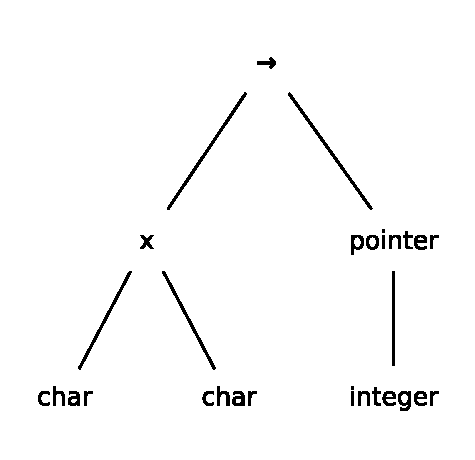
\includegraphics[width=0.3\textwidth]{img/36.pdf}}
\end{figure}

\subsubsection{DAG}
\begin{figure}[H]
    \centerline{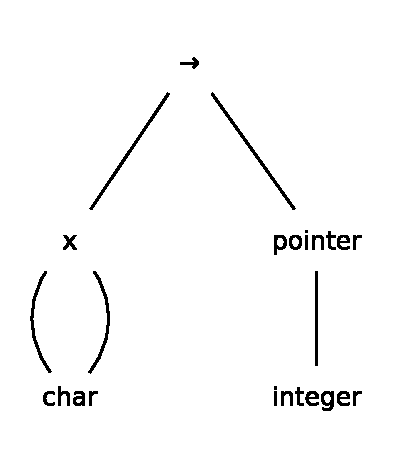
\includegraphics[width=0.3\textwidth]{img/37.pdf}}
\end{figure}

\subsection{Constructions of Type Expressions}

\subsection{Types Names}

\subsection{Name Equivalence}

\subsection{Type Checker}


\section{Symbol Table}

\subsection{Designing a Symbol Table}

\subsection{Type Expression}

\subsubsection{Implementing Type Expressions}

\section{Type Checker}
\subsection{Semantic}

\subsection{Complete Grammar}

